\subsection{Türk İslâm Eserleri Müzesi}
\begin{wrapfigure}{r}{0.4\textwidth}
    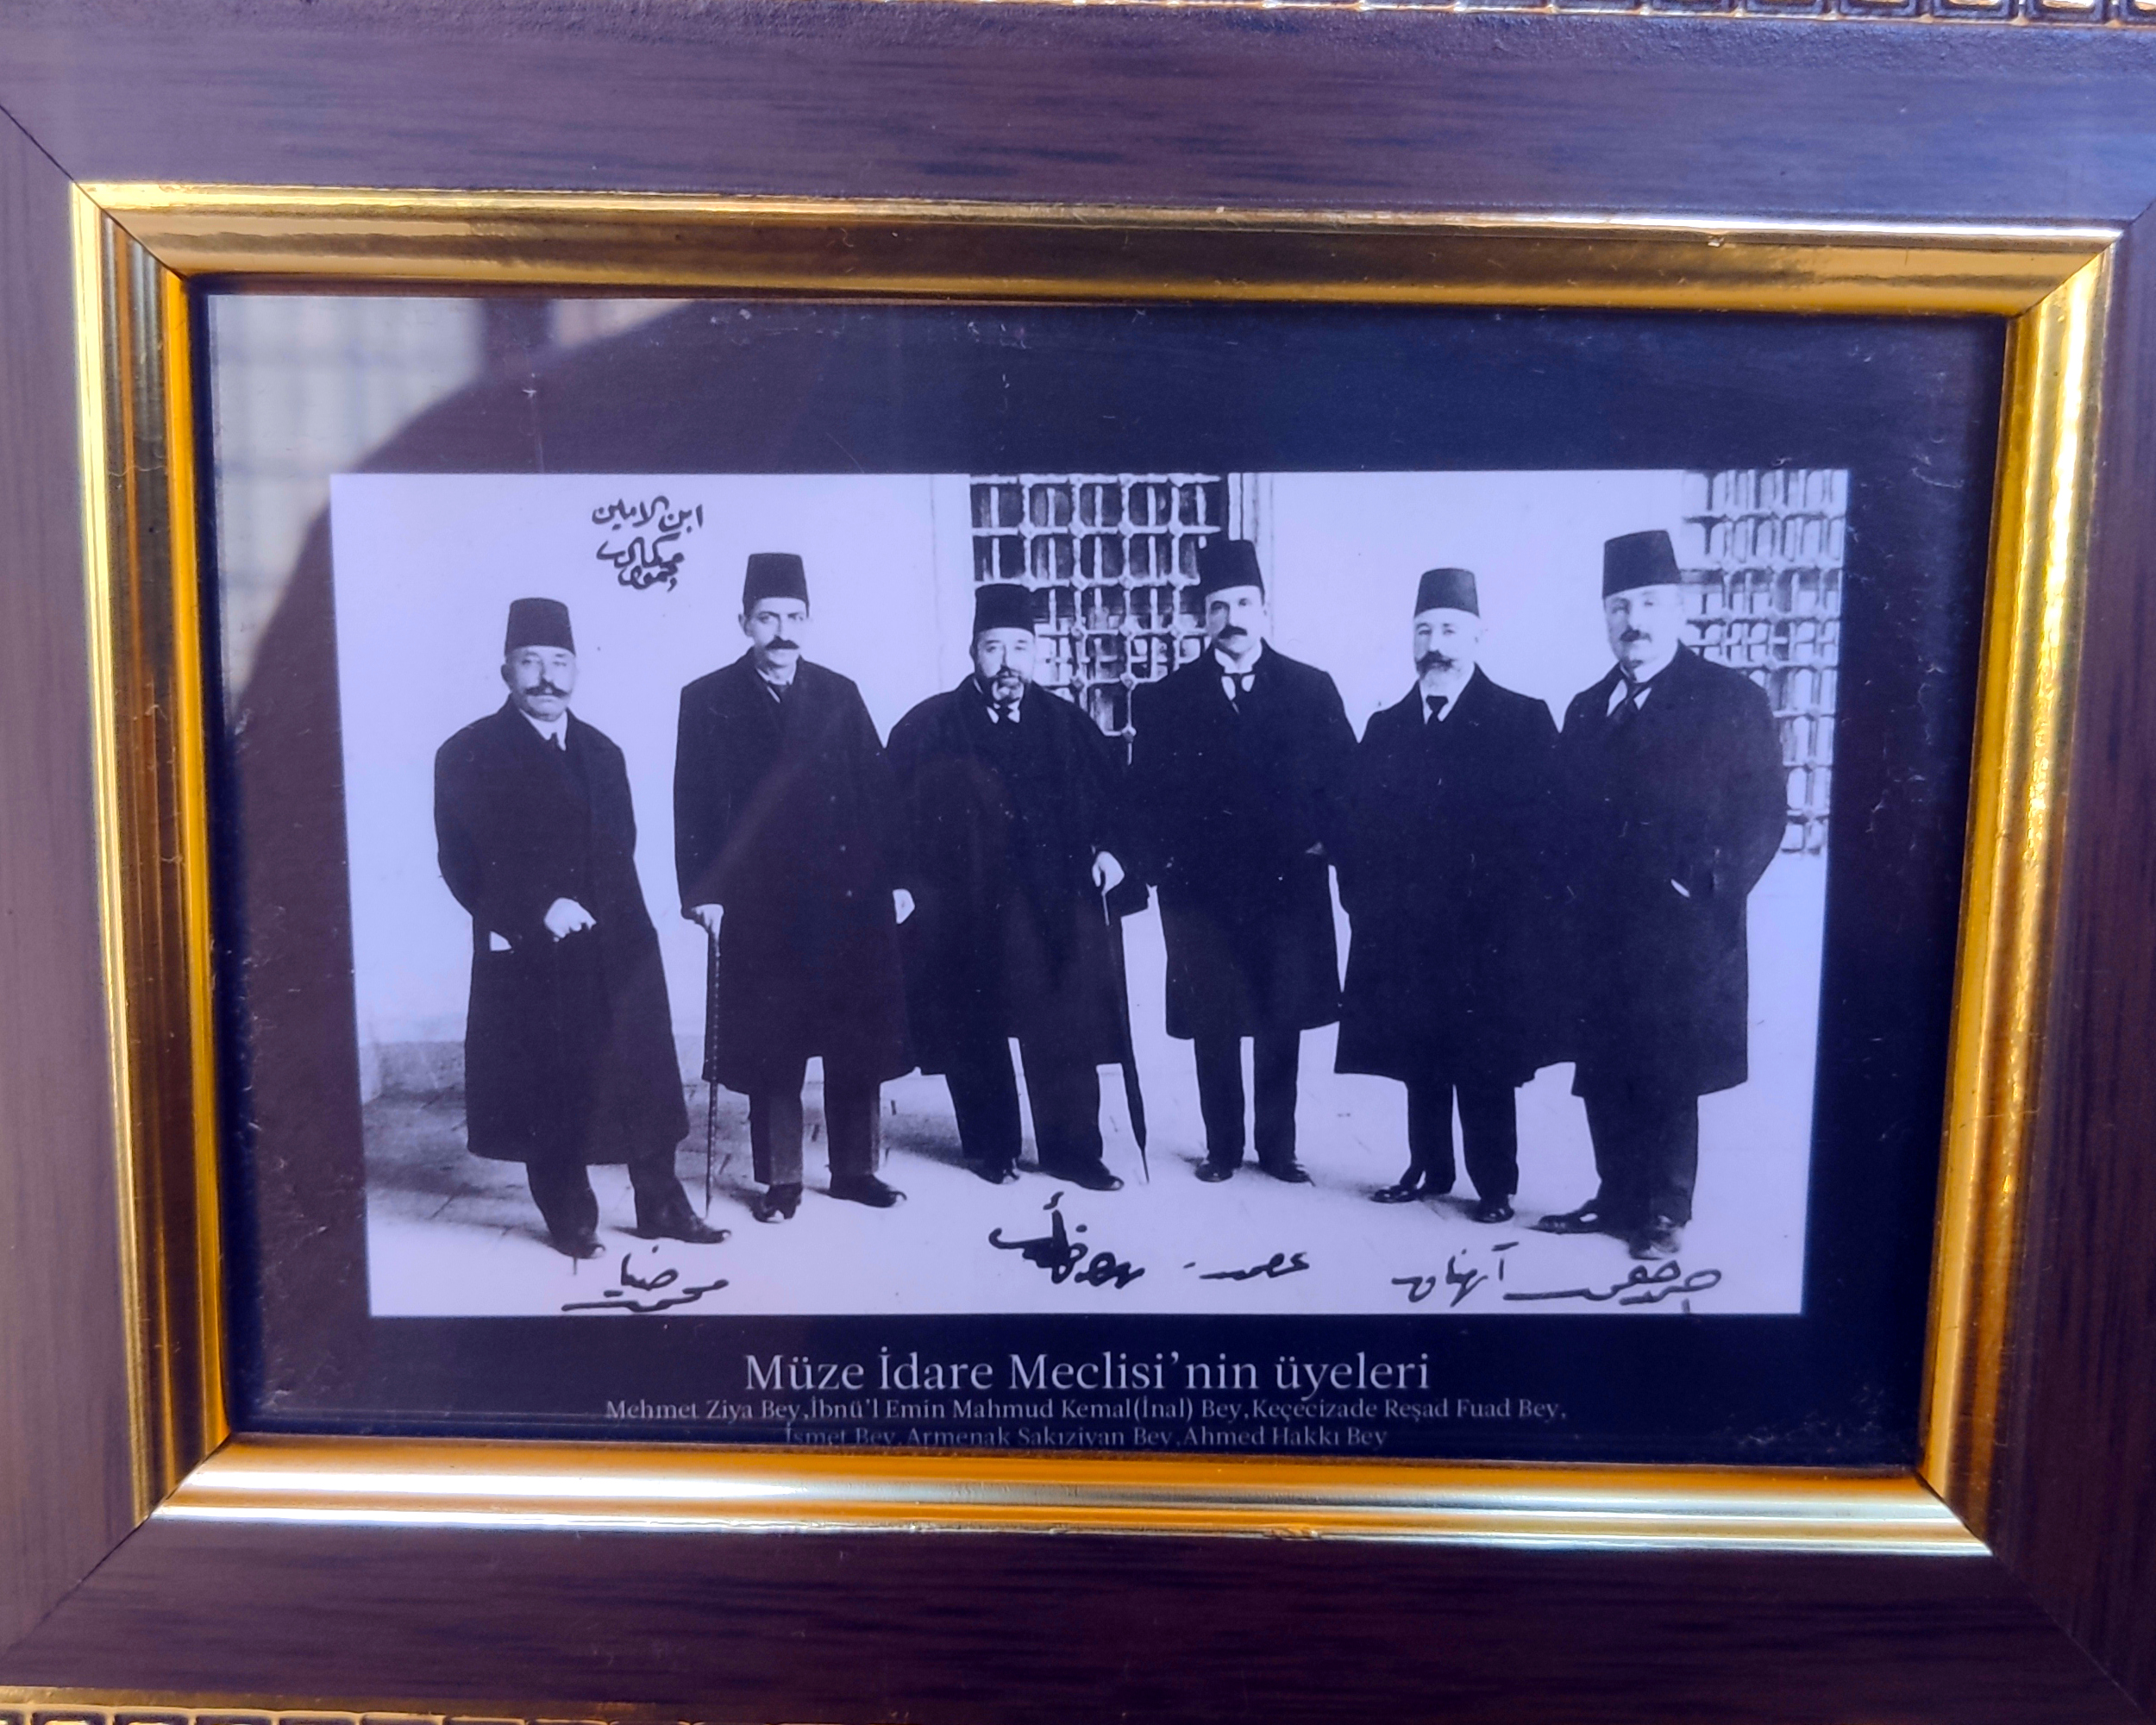
\includegraphics[width=0.4\textwidth]{assets/museum_opening.jpg}
    \caption{Müze Açılışında Bir Fotoğraf}
    \label{fig:musem_opening}
\end{wrapfigure}
\indent\indent 1908 yılından itibaren yapılan toplantılarda Sadrazamlık, Maarif Nezareti ve Müze-i Hümâyun kurumları, kıymetli eşyların yurt dışına çıkarılmasını engellemek için Hazîne-i Evkaf-ı Hümâyun İdaresi'ne bağlı bir müzede koruma altına alınmasını önermiştir. Yine aynı dönemde Sadrazam Hüseyin Hilmi Paşa'nın imzasını taşıyan tezkereler, eski eserlerin yurt dışına çıkışını engellemek için gümrüklere gönderilmiştir. Bu girişimlerin sonucunda Türk İslâm Eserleri Müzesi, 1914 yılında Evkaf-ı İslâmiyye Müzesi ismiyle Süleymaniye Camii'nin imarethanesinde kurulmuştur. Müze, 27 Nisan 1914 tarihinde, Sultan Mehmed Reşat'ın tahta çıkışının yıldönümünde açılmıştır. Açılışta Veliaht Yusuf İzettin Efendi, Sadrazam Said Halim Paşa, Şeyhülislâm Ürgüplü Hayri Efendi, Besim Ömer Paşa hazır bulunmuşlardır. Kuruluşunda Evkaf-ı Humâyun Nezareti'ne bağlı olan müze, 1924 yılında bu nezaretin kaldırılmasıyla Maarif Vekaleti'ne bağlanmıştır. Zaman içinde artan eski eserlerden dolayı, Süleymaniye Camii'nin imarethanesi yetersiz kalmış ve 1983 yılında Sultanahmet'teki İbrahim Paşa Sarayı'na taşınmıştır.\cite{dia_2}\newline
\indent İbrahim Paşa Sarayı'nın inşa tarihi bilinmemektedir. II.Bayezid döneminde yaşamış tarihçi Solakzade, At Meydanı'nda inşa edilen bir saraydan bahsetmektedir.\cite{atasoy_1} Saraya dair ilk yazılı belge 1521 yılına ait. Bu belge, mevcut sarayın tamiratını buyurmaktadır. Dört avlu, ahırlar, bir kule ve hazine binasından oluşan saray, oldukça geniş bir araziye yayılmış durumdaydı. İbrahim Paşa'nın, 1524 yılında 15gün süren düğünü yine bu sarayda yapılmıştır. İbrahim Paşa'nın 1536'daki idamı üzerinde saray müsadere edilmiştir. Sonraki dönemlerde de saray sadrazamlara, vezirlere ve önemli devlet adamlarına tahsis edilmiştir. 1652 yılında yanan saray, 1720 civarında Nevşehirli Damat İbrahim Paşa tarafından tamir ettirilmiştir. 1741'te tekrar yanan saray bir daha onarılmamıştır.\cite{dia_3} Sarayın üçüncü avlusuna 1910 yılında Mimar Vedat Tek'in projelendirdiği Defter-i Hakani(Tapu Kadastro Müdürlüğü)(günümüzde Ayasofya Müzesi) binası yapılmıştır. Sarayın bir diğer avlusu ise 1939 yılında Adliye Sarayı'nın inşası için yıkılmıştır. 1970lerde restorasyon geçiren sarayın ikinci avlusu, 1983 yılında Türk İslâm Eserleri Müzesi'ne tahsis edilmiştir.\cite{atasoy_2}